\documentclass[10pt,twocolumn]{article}

\usepackage[T1]{fontenc}
\usepackage[utf8]{inputenc}
\usepackage{lmodern}
\usepackage[a4paper,margin=0.72in,top=0.72in,bottom=0.82in]{geometry}
\usepackage{microtype}
\usepackage{amsmath,amssymb}
\usepackage{booktabs}
\usepackage{tabularx}
\usepackage{array}
\usepackage{xcolor}
\usepackage{graphicx}
\usepackage{caption}
\usepackage{enumitem}
\usepackage{listings}
\usepackage{hyperref}
\usepackage{tikz}
\usepackage{pgfplots}
\usepackage{titlesec}
\usepackage{fancyhdr}

\pgfplotsset{compat=1.18}
\usetikzlibrary{
  arrows.meta, positioning, calc, fit, backgrounds,
  shapes.geometric, shapes.misc, decorations.pathreplacing
}

\definecolor{blueA}{HTML}{1D4ED8}
\definecolor{blueB}{HTML}{DBEAFE}
\definecolor{violetA}{HTML}{6D28D9}
\definecolor{violetB}{HTML}{EDE9FE}
\definecolor{greenA}{HTML}{047857}
\definecolor{greenB}{HTML}{D1FAE5}
\definecolor{orangeA}{HTML}{B45309}
\definecolor{orangeB}{HTML}{FEF3C7}
\definecolor{redA}{HTML}{B91C1C}
\definecolor{redB}{HTML}{FEE2E2}
\definecolor{grayA}{HTML}{374151}
\definecolor{grayB}{HTML}{F3F4F6}
\definecolor{ink}{HTML}{111827}
\definecolor{codebg}{HTML}{F8FAFC}

\hypersetup{
  colorlinks=true,
  linkcolor=blueA,
  urlcolor=blueA,
  citecolor=blueA,
  pdftitle={DiffuSVG: Diffusion-Guided Reinforcement Learning for SVG Generation},
  pdfauthor={}
}

\pagestyle{fancy}
\fancyhf{}
\fancyhead[L]{\footnotesize DiffuSVG}
\fancyhead[R]{\footnotesize Diffusion-guided SVG generation}
\fancyfoot[C]{\footnotesize\thepage}
\renewcommand{\headrulewidth}{0.3pt}

\titleformat{\section}
  {\large\bfseries\color{ink}}{\thesection}{0.6em}{}
\titleformat{\subsection}
  {\normalsize\bfseries\color{ink}}{\thesubsection}{0.55em}{}
\titleformat{\subsubsection}
  {\normalsize\itshape\color{ink}}{\thesubsubsection}{0.5em}{}
\titlespacing*{\section}{0pt}{1.2ex plus .2ex}{0.7ex}
\titlespacing*{\subsection}{0pt}{0.9ex plus .2ex}{0.35ex}

\setlist[itemize]{leftmargin=*,topsep=2pt,itemsep=1pt}
\setlist[enumerate]{leftmargin=*,topsep=2pt,itemsep=1pt}
\setlength{\columnsep}{0.23in}
\raggedbottom

\lstset{
  basicstyle=\ttfamily\scriptsize,
  backgroundcolor=\color{codebg},
  frame=single,
  framerule=0.3pt,
  rulecolor=\color{gray!35},
  breaklines=true,
  columns=fullflexible,
  showstringspaces=false,
  tabsize=2,
  xleftmargin=4pt,
  xrightmargin=4pt,
  aboveskip=4pt,
  belowskip=4pt
}

\newcommand{\pith}{\pi_{\theta}}
\newcommand{\piref}{\pi_{\mathrm{ref}}}
\newcommand{\render}{\mathcal{R}}
\newcommand{\clip}{\mathrm{CLIP}}

\tikzset{
  proc/.style={
    draw=#1, fill=#1!10, rounded corners=4pt,
    line width=0.7pt, align=center, inner sep=5pt,
    minimum height=0.78cm, font=\scriptsize
  },
  data/.style={
    draw=orangeA, fill=orangeB, rounded corners=3pt,
    line width=0.65pt, align=center, inner sep=4pt,
    minimum height=0.65cm, font=\scriptsize
  },
  model/.style={
    draw=greenA, fill=greenB, rounded corners=4pt,
    line width=0.8pt, align=center, inner sep=5pt,
    minimum height=0.78cm, font=\scriptsize\bfseries
  },
  reward/.style={
    draw=violetA, fill=violetB, rounded corners=4pt,
    line width=0.75pt, align=center, inner sep=5pt,
    minimum height=0.75cm, font=\scriptsize
  },
  arrow/.style={-{Stealth[length=2.1mm]}, line width=0.75pt},
  dashedarrow/.style={-{Stealth[length=2.1mm]}, line width=0.65pt, dashed, color=orangeA},
  stage/.style={draw=#1, fill=#1!5, rounded corners=8pt, dashed, inner sep=8pt}
}

\begin{document}

\makeatletter
\twocolumn[
\begin{@twocolumnfalse}
\begin{center}
{\LARGE\bfseries DiffuSVG: Diffusion-Guided Reinforcement Learning\\[-1pt]
for Complex Scene SVG Generation\par}
\vspace{0.85em}
\end{center}

\begin{abstract}
Text-to-SVG generation is a structured generation problem: a model must emit
valid XML code whose rendered image matches a natural-language scene. General
vision-language models can produce SVG snippets, but they often collapse on
complex prompts, drawing one salient object repeatedly instead of composing a
scene. We present \textbf{DiffuSVG}, a two-stage pipeline that first teaches SVG
syntax with supervised fine-tuning and preference optimization, then improves
visual fidelity with diffusion-guided group reinforcement learning. The system
uses a plan-then-draw prompting format, synthetic SVG supervision, DPO
preference pairs, Stable Diffusion reference images, and a CLIP-based reward
augmented with an element-count bonus. The final pipeline trains Qwen2.5-VL-7B
with LoRA on a single A100 GPU and is designed to improve medium and complex
multi-object SVG scenes while remaining fully reproducible from scripts.
\end{abstract}

\vspace{0.35em}
\noindent\textbf{Keywords:} SVG generation, vector graphics, diffusion guidance,
reinforcement learning, GRPO, DPO, CLIP reward, LoRA.
\vspace{1.0em}
\end{@twocolumnfalse}
]
\makeatother

\section{Introduction}

Scalable Vector Graphics (SVG) represent images as XML-defined geometric
elements such as rectangles, ellipses, polygons, and Bezier paths. This makes
SVGs resolution-independent, editable, and compact. However, it also makes
text-to-SVG generation harder than raster image synthesis. The output must be
valid code, visually meaningful after rendering, and geometrically organized.

Modern vision-language models have enough web knowledge to emit SVG code, but
their complex-scene behavior is brittle. In early experiments, prompts such as
``a beach at dawn with waves, clouds, and a lighthouse'' often produced many
concentric circles for the sun while omitting the sea, beach, and lighthouse.
We refer to this as \emph{object fixation}: the model begins drawing one
salient object and fails to allocate tokens to the rest of the scene.

DiffuSVG addresses this failure mode by combining three ideas. First, the
model is prompted to plan the scene before writing SVG code. Second, syntax is
learned separately from visual alignment through SFT and DPO. Third, complex
scene quality is improved with GRPO against diffusion-generated reference
images, where CLIP evaluates rendered SVGs instead of raw code.

\paragraph{Contributions.}
This paper describes:
\begin{itemize}
  \item a reproducible two-stage training pipeline for text-to-SVG generation;
  \item a plan-then-draw prompt that reduces object fixation in complex scenes;
  \item a synthetic SFT and DPO pipeline requiring no human-labeled SVG corpus;
  \item a diffusion-guided GRPO stage using CLIP-I, CLIP-T, and element-count
        rewards;
  \item an implementation designed for a single NVIDIA A100 GPU.
\end{itemize}

\section{Pipeline Overview}

The method separates SVG generation into two learning problems. Stage 1 teaches
the model to produce valid, colorful SVG code. Stage 2 teaches the model to make
rendered SVGs visually match complex scene prompts.

\begin{figure*}[t]
\centering
\resizebox{\textwidth}{!}{
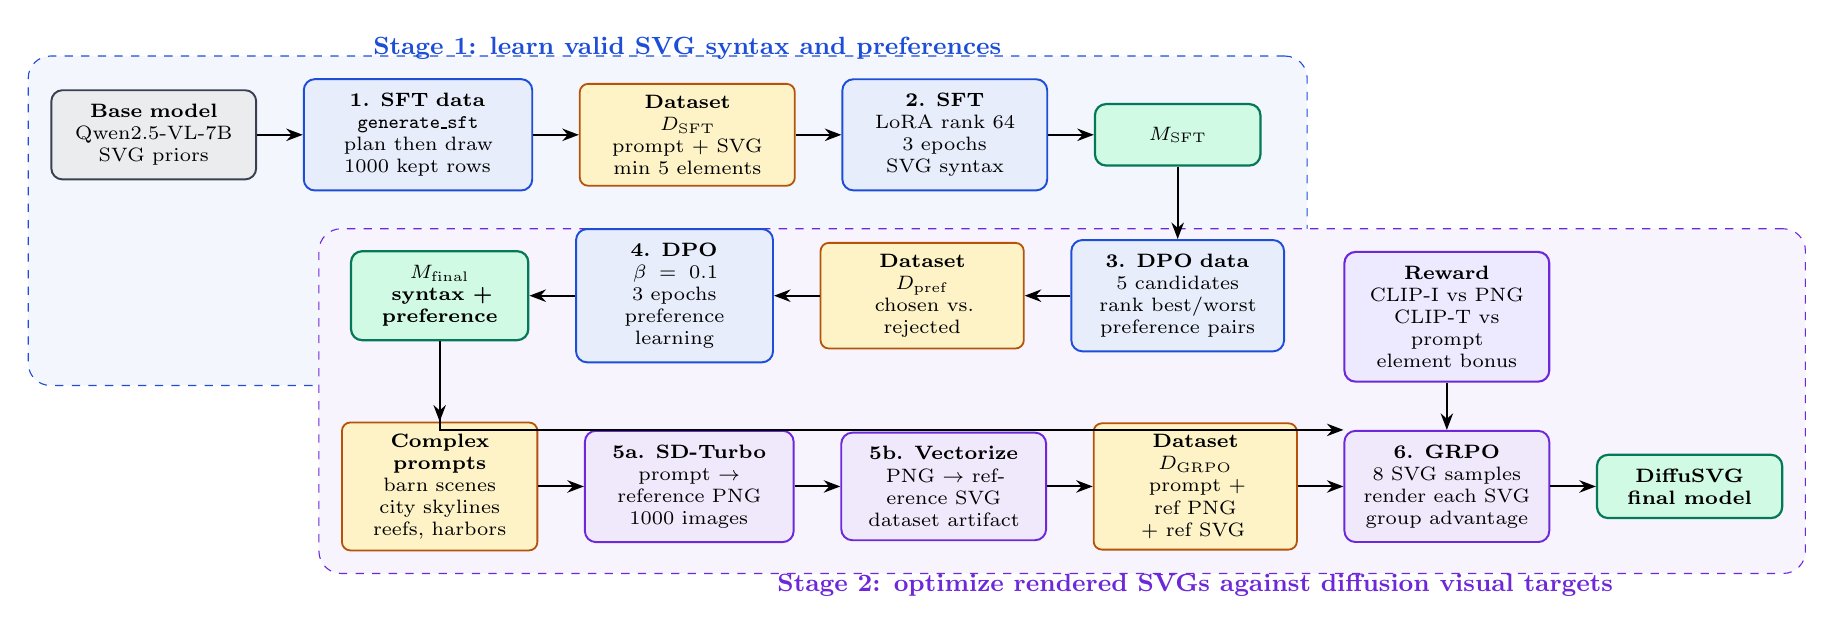
\begin{tikzpicture}[node distance=0.55cm and 0.58cm]
  \node[proc=grayA, text width=2.25cm] (base)
    {\textbf{Base model}\\Qwen2.5-VL-7B\\SVG priors};
  \node[proc=blueA, right=of base, text width=2.55cm] (step1)
    {\textbf{1. SFT data}\\\texttt{generate\_sft}\\plan then draw\\1000 kept rows};
  \node[data, right=of step1, text width=2.45cm] (dsft)
    {\textbf{Dataset}\\$D_{\mathrm{SFT}}$\\prompt + SVG\\min 5 elements};
  \node[proc=blueA, right=of dsft, text width=2.25cm] (step2)
    {\textbf{2. SFT}\\LoRA rank 64\\3 epochs\\SVG syntax};
  \node[model, right=of step2, text width=1.75cm] (msft)
    {$M_{\mathrm{SFT}}$};

  \node[proc=blueA, below=0.92cm of msft, text width=2.35cm] (step3)
    {\textbf{3. DPO data}\\5 candidates\\rank best/worst\\preference pairs};
  \node[data, left=of step3, text width=2.3cm] (dpref)
    {\textbf{Dataset}\\$D_{\mathrm{pref}}$\\chosen vs. rejected};
  \node[proc=blueA, left=of dpref, text width=2.15cm] (step4)
    {\textbf{4. DPO}\\$\beta=0.1$\\3 epochs\\preference learning};
  \node[model, left=of step4, text width=1.9cm] (mfinal)
    {$M_{\mathrm{final}}$\\syntax + preference};

  \node[data, below=1.02cm of mfinal, text width=2.2cm] (prompts)
    {\textbf{Complex prompts}\\barn scenes\\city skylines\\reefs, harbors};
  \node[proc=violetA, right=of prompts, text width=2.3cm] (step5a)
    {\textbf{5a. SD-Turbo}\\prompt $\to$ reference PNG\\1000 images};
  \node[proc=violetA, right=of step5a, text width=2.25cm] (step5b)
    {\textbf{5b. Vectorize}\\PNG $\to$ reference SVG\\dataset artifact};
  \node[data, right=of step5b, text width=2.3cm] (dgrpo)
    {\textbf{Dataset}\\$D_{\mathrm{GRPO}}$\\prompt + ref PNG\\+ ref SVG};
  \node[proc=violetA, right=of dgrpo, text width=2.25cm] (step6)
    {\textbf{6. GRPO}\\8 SVG samples\\render each SVG\\group advantage};
  \node[model, right=of step6, text width=2.0cm] (out)
    {DiffuSVG\\final model};

  \node[reward, above=0.6cm of step6, text width=2.25cm] (reward)
    {\textbf{Reward}\\CLIP-I vs PNG\\CLIP-T vs prompt\\element bonus};

  \draw[arrow] (base) -- (step1);
  \draw[arrow] (step1) -- (dsft);
  \draw[arrow] (dsft) -- (step2);
  \draw[arrow] (step2) -- (msft);
  \draw[arrow] (msft) -- (step3);
  \draw[arrow] (step3) -- (dpref);
  \draw[arrow] (dpref) -- (step4);
  \draw[arrow] (step4) -- (mfinal);
  \draw[arrow] (mfinal) -- (prompts);
  \draw[arrow] (prompts) -- (step5a);
  \draw[arrow] (step5a) -- (step5b);
  \draw[arrow] (step5b) -- (dgrpo);
  \draw[arrow] (dgrpo) -- (step6);
  \draw[arrow] (reward) -- (step6);
  \draw[arrow] (step6) -- (out);
  \draw[arrow] (mfinal.south) |- (step6.north west);

  \begin{scope}[on background layer]
    \node[stage=blueA, fit=(base)(step1)(dsft)(step2)(msft)(step3)(dpref)(step4)(mfinal)] {};
    \node[stage=violetA, fit=(prompts)(step5a)(step5b)(dgrpo)(reward)(step6)(out)] {};
  \end{scope}

  \node[font=\bfseries\small\color{blueA}, above=0.18cm of dsft]
    {Stage 1: learn valid SVG syntax and preferences};
  \node[font=\bfseries\small\color{violetA}, below=0.18cm of dgrpo]
    {Stage 2: optimize rendered SVGs against diffusion visual targets};
\end{tikzpicture}}
\caption{Detailed DiffuSVG pipeline. The upper stage builds a valid SVG model
through SFT and DPO. The lower stage creates diffusion references and uses GRPO
to optimize rendered SVGs for complex scene prompts. Each box shows the script
role, training signal, or produced dataset artifact.}
\label{fig:pipeline}
\end{figure*}

Figure~\ref{fig:pipeline} shows the full training flow. The intermediate
artifact \(M_{\mathrm{final}}\) is already a useful SVG generator; the GRPO
stage further optimizes it for visual agreement with reference images.

\begin{figure*}[t]
\centering
\resizebox{0.96\textwidth}{!}{
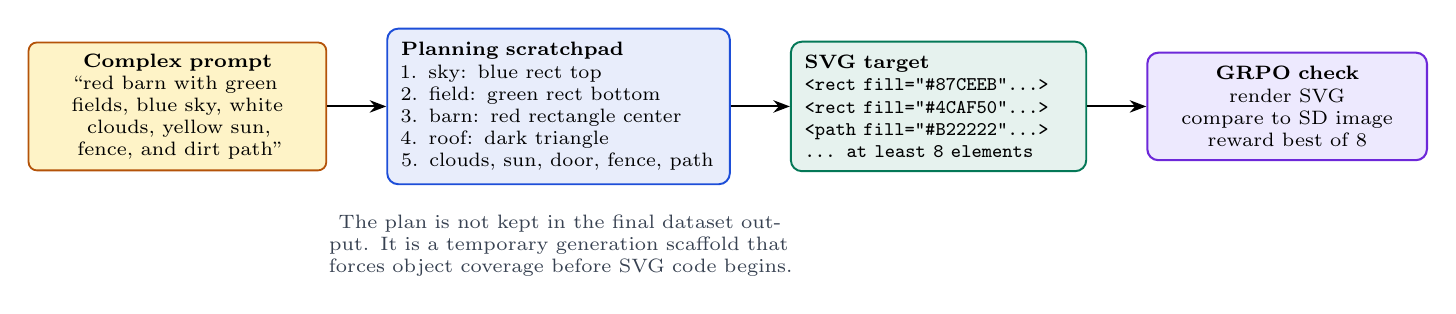
\begin{tikzpicture}[node distance=0.7cm and 0.75cm]
  \node[data, text width=3.5cm] (prompt)
    {\textbf{Complex prompt}\\``red barn with green fields, blue sky,
    white clouds, yellow sun, fence, and dirt path''};
  \node[proc=blueA, right=of prompt, text width=4.0cm, align=left] (plan)
    {\textbf{Planning scratchpad}\\
    1. sky: blue rect top\\
    2. field: green rect bottom\\
    3. barn: red rectangle center\\
    4. roof: dark triangle\\
    5. clouds, sun, door, fence, path};
  \node[proc=greenA, right=of plan, text width=3.4cm, align=left] (svg)
    {\textbf{SVG target}\\
    \texttt{<rect fill="\#87CEEB"...>}\\
    \texttt{<rect fill="\#4CAF50"...>}\\
    \texttt{<path fill="\#B22222"...>}\\
    \texttt{... at least 8 elements}};
  \node[reward, right=of svg, text width=3.2cm] (rewarded)
    {\textbf{GRPO check}\\render SVG\\compare to SD image\\reward best of 8};

  \draw[arrow] (prompt) -- (plan);
  \draw[arrow] (plan) -- (svg);
  \draw[arrow] (svg) -- (rewarded);

  \node[below=0.25cm of plan, font=\scriptsize\color{grayA}, text width=8.5cm, align=center]
    {The plan is not kept in the final dataset output. It is a temporary
    generation scaffold that forces object coverage before SVG code begins.};
\end{tikzpicture}}
\caption{Worked example for a complex prompt. The same prompt pattern is used
in SFT generation, DPO candidate generation, GRPO sampling, and inference.}
\label{fig:worked-example}
\end{figure*}

\section{Method}

\subsection{Plan-then-draw Prompting}

The central prompt design is simple: before emitting SVG code, the model must
list every major object, its approximate location on a \(200\times200\) canvas,
and its color. Only after this plan does it draw the SVG. The regex extractor
keeps only the \texttt{<svg>...</svg>} block, so the plan guides
generation without becoming part of the training target.

\begin{figure}[t]
\centering
\resizebox{\linewidth}{!}{
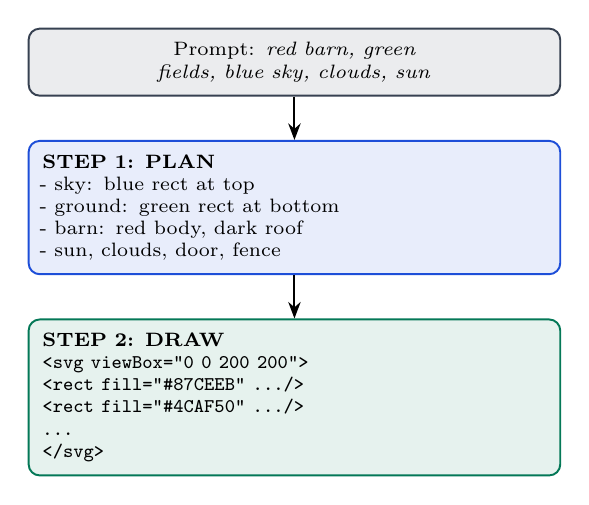
\begin{tikzpicture}[node distance=0.55cm]
  \node[proc=grayA, text width=6.4cm] (prompt) {
    Prompt: \textit{red barn, green fields, blue sky, clouds, sun}
  };
  \node[proc=blueA, below=of prompt, text width=6.4cm, align=left] (plan) {
    \textbf{STEP 1: PLAN}\\
    - sky: blue rect at top\\
    - ground: green rect at bottom\\
    - barn: red body, dark roof\\
    - sun, clouds, door, fence
  };
  \node[proc=greenA, below=of plan, text width=6.4cm, align=left] (svg) {
    \textbf{STEP 2: DRAW}\\
    \texttt{<svg viewBox="0 0 200 200">}\\
    \texttt{<rect fill="\#87CEEB" .../>}\\
    \texttt{<rect fill="\#4CAF50" .../>}\\
    \texttt{...}\\
    \texttt{</svg>}
  };
  \draw[arrow] (prompt) -- (plan);
  \draw[arrow] (plan) -- (svg);
\end{tikzpicture}}
\caption{Plan-then-draw prompting. Planning acts as a scratchpad that commits
the model to multiple objects before it starts producing SVG tokens.}
\label{fig:cot}
\end{figure}

This directly targets object fixation. The model is less likely to spend all
tokens on a single sun, tree, or flower because the plan has already exposed the
expected scene inventory.

\subsection{Synthetic SFT Data}

No curated SVG dataset is assumed. Instead, the base Qwen2.5-VL model generates
its own supervised examples from a prompt pool containing simple, medium, and
complex scenes. Each output is standardized and filtered before being saved.

\begin{equation}
D_{\mathrm{SFT}} =
\{(x_i, y_i): y_i = \mathrm{Filter}(\mathrm{Std}(\mathrm{Qwen}(x_i)))\}.
\end{equation}

The filter keeps an SVG only if it contains:
\begin{itemize}
  \item a valid \texttt{<svg>} root and closing tag;
  \item at least five filled elements;
  \item a canonical \texttt{viewBox="0 0 200 200"};
  \item visible color attributes.
\end{itemize}

The element threshold intentionally rejects sparse outputs such as a background
and two blobs. This improves the training signal for complex scenes.

\subsection{Supervised Fine-Tuning}

The SFT stage trains a LoRA adapter on \(D_{\mathrm{SFT}}\). For target sequence
\(y=(y_1,\ldots,y_T)\) and prompt \(x\), the loss is standard next-token
negative log likelihood:

\begin{equation}
\mathcal{L}_{\mathrm{SFT}}(\theta)
= -\sum_{t=1}^{T} \log p_{\theta}(y_t \mid x,y_{<t}).
\end{equation}

LoRA reduces memory usage by freezing base weights and learning a low-rank
update:

\begin{equation}
W' = W + \Delta W,\qquad
\Delta W = \frac{\alpha}{r}BA,
\end{equation}

where \(r=64\) and \(\alpha=128\). This makes the method feasible on a single
A100 while preserving the base model's broad language and code knowledge.

\subsection{Direct Preference Optimization}

SFT improves syntax but does not guarantee visual quality. Therefore, the
\(M_{\mathrm{SFT}}\) model generates five candidates per prompt. A scoring
function ranks candidates by renderability, color, element count, and prompt
coverage. The best and worst candidates form DPO pairs.

\begin{figure}[t]
\centering
\resizebox{\linewidth}{!}{
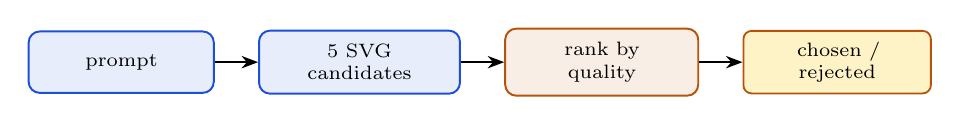
\begin{tikzpicture}[node distance=0.55cm and 0.55cm]
  \node[proc=blueA, text width=2.0cm] (prompt) {prompt};
  \node[proc=blueA, right=of prompt, text width=2.2cm] (cand) {5 SVG\\candidates};
  \node[proc=orangeA, right=of cand, text width=2.1cm] (rank) {rank by\\quality};
  \node[data, right=of rank, text width=2.1cm] (pair) {chosen /\\rejected};
  \draw[arrow] (prompt) -- (cand);
  \draw[arrow] (cand) -- (rank);
  \draw[arrow] (rank) -- (pair);
\end{tikzpicture}}
\caption{DPO dataset construction. Five candidates produce richer preference
pairs than the three-candidate baseline.}
\label{fig:dpo}
\end{figure}

DPO optimizes the probability of the preferred SVG \(y_w\) over the rejected
SVG \(y_l\):

\begin{equation}
\mathcal{L}_{\mathrm{DPO}} =
-\log \sigma\left(
\beta
\left[
\log\frac{\pith(y_w|x)}{\piref(y_w|x)}
-
\log\frac{\pith(y_l|x)}{\piref(y_l|x)}
\right]
\right),
\end{equation}

with \(\beta=0.1\). This stage yields \(M_{\mathrm{final}}\), the starting point
for diffusion-guided reinforcement learning.

\subsection{Diffusion-Guided GRPO}

Stage 2 creates visual targets for complex prompts. SD-Turbo generates a
reference PNG for each prompt. The PNG is vectorized into a reference SVG for
dataset completeness, but the reward primarily compares the rendered candidate
SVG to the reference PNG.

For each prompt \(x\), GRPO samples \(n=8\) SVG candidates from the current
policy. Each SVG is rendered to a bitmap using CairoSVG. Rewards are computed
from rendered images, not code strings:

\begin{equation}
\begin{aligned}
r(y,x,I_{\mathrm{ref}}) ={}&
0.45\,s_I(\render(y), I_{\mathrm{ref}}) \\
&+ 0.40\,s_T(\render(y), x)
+ 0.15\,b_{\mathrm{elem}}(y).
\end{aligned}
\end{equation}

where \(s_I\) is CLIP image-image similarity, \(s_T\) is CLIP text-image
similarity, and \(b_{\mathrm{elem}}\) rewards a sufficient number of distinct
filled elements. The CLIP backbone is upgraded to ViT-L/14 for stronger visual
judgment.

\begin{figure}[t]
\centering
\resizebox{\linewidth}{!}{
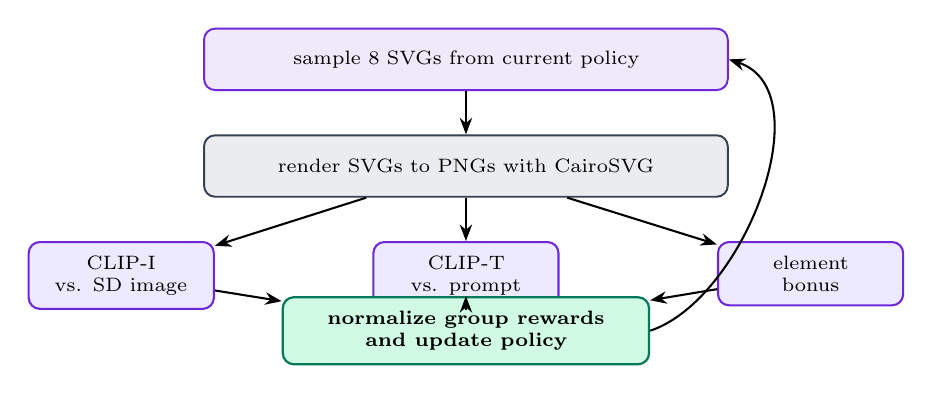
\begin{tikzpicture}[node distance=0.55cm]
  \node[proc=violetA, text width=6.3cm] (sample) {
    sample 8 SVGs from current policy
  };
  \node[proc=grayA, below=of sample, text width=6.3cm] (render) {
    render SVGs to PNGs with CairoSVG
  };
  \node[reward, below left=0.55cm and -0.15cm of render, text width=2.0cm] (ci) {CLIP-I\\vs. SD image};
  \node[reward, below=0.55cm of render, text width=2.0cm] (ct) {CLIP-T\\vs. prompt};
  \node[reward, below right=0.55cm and -0.15cm of render, text width=2.0cm] (eb) {element\\bonus};
  \node[model, below=1.25cm of render, text width=4.3cm] (update) {
    normalize group rewards\\and update policy
  };
  \draw[arrow] (sample) -- (render);
  \draw[arrow] (render) -- (ci);
  \draw[arrow] (render) -- (ct);
  \draw[arrow] (render) -- (eb);
  \draw[arrow] (ci) -- (update);
  \draw[arrow] (ct) -- (update);
  \draw[arrow] (eb) -- (update);
  \draw[arrow] (update.east) .. controls +(1.2,0.4) and +(1.2,-0.4) .. (sample.east);
\end{tikzpicture}}
\caption{GRPO reward loop. SVG candidates are rendered before scoring, making
the reward visual rather than purely syntactic.}
\label{fig:grpo}
\end{figure}

For candidate \(i\), the group-relative advantage is

\begin{equation}
A_i = \frac{r_i-\bar r}{\sigma_r+\epsilon},\qquad
\bar r = \frac{1}{n}\sum_{j=1}^{n} r_j.
\end{equation}

This turns each group of candidates into an internal comparison set. The model
learns which SVGs are better for the same prompt without requiring absolute
human labels.

\section{Datasets and Artifacts}

The project uses generated datasets rather than external human-labeled SVG
corpora. This keeps the pipeline reproducible and avoids manual annotation.

\begin{table}[t]
\centering
\caption{Datasets produced by the pipeline.}
\label{tab:datasets}
\begin{tabularx}{\linewidth}{@{}l>{\raggedright\arraybackslash}Xr@{}}
\toprule
\textbf{Dataset} & \textbf{Role} & \textbf{Size} \\
\midrule
\(D_{\mathrm{SFT}}\) &
Conversation-format SVG examples generated by the base model and filtered for
validity, color, and element count. & 1000 \\
\(D_{\mathrm{pref}}\) &
Chosen/rejected SVG pairs built from five candidates per prompt. & 1500 prompts \\
\(D_{\mathrm{GRPO}}\) &
Complex prompts with SD-Turbo reference PNGs and vectorized SVG artifacts. & 1000 \\
\bottomrule
\end{tabularx}
\end{table}

The SFT generator uses temperature sampling rather than greedy decoding. Greedy
decoding produced repeated templates; sampling increases diversity and gives
DPO a broader candidate distribution.

\section{Implementation Details}

The implementation is organized as a clean repository with two stage folders:

\begin{lstlisting}[language=bash]
DiffuSVG/
  train.sh
  infer.py
  prompts.txt
  stage1/
    generate_sft_data.py
    build_dpo_data.py
    dpo_train.py
    svg_utils.py
  stage2/
    filter_prompts.py
    generate_pngs.py
    vectorize_svgs.py
    build_dataset.py
    grpo_train.py
    rewards.py
\end{lstlisting}

The whole run is launched with:

\begin{lstlisting}[language=bash]
bash train.sh prompts.txt
\end{lstlisting}

\begin{table}[t]
\centering
\caption{Final training configuration.}
\label{tab:hparams}
\begin{tabularx}{\linewidth}{@{}lX@{}}
\toprule
\textbf{Component} & \textbf{Setting} \\
\midrule
Base model & Qwen2.5-VL-7B-Instruct \\
SFT samples & 1000 \\
SFT LoRA & rank 64, alpha 128, 3 epochs \\
DPO candidates & 5 per prompt \\
DPO beta & 0.1 \\
Reference generator & SD-Turbo \\
Reward backbone & CLIP ViT-L/14 \\
GRPO samples & 8 per prompt \\
GRPO beta & 0.04 \\
Hardware & single NVIDIA A100 \\
Estimated runtime & about 65 hours \\
\bottomrule
\end{tabularx}
\end{table}

\section{Evaluation Protocol}

The training run is designed to compare four checkpoints:
\[
M_0,\quad M_{\mathrm{SFT}},\quad M_{\mathrm{final}},\quad
M_{\mathrm{GRPO}}.
\]
The recommended evaluation set contains simple object prompts, medium
multi-object prompts, and complex scenes. Each checkpoint is evaluated by
rendering generated SVGs and computing CLIP-T, CLIP-I against diffusion
references, render success rate, and element count.

\begin{figure}[t]
\centering
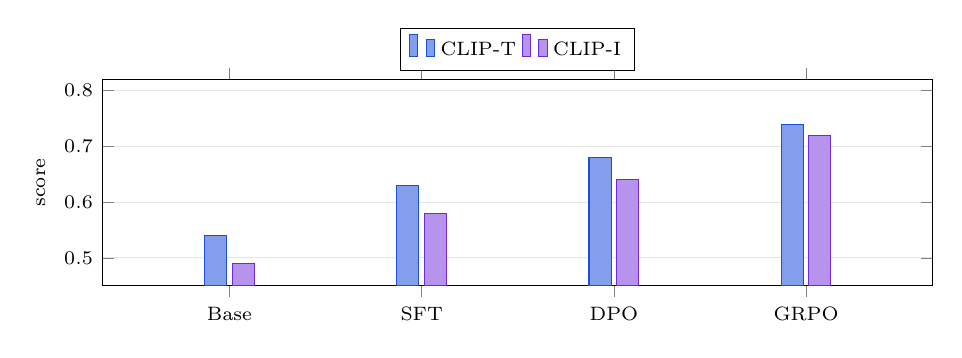
\begin{tikzpicture}
\begin{axis}[
  ybar,
  width=\linewidth,
  height=4.2cm,
  ymin=0.45, ymax=0.82,
  ylabel={score},
  symbolic x coords={Base,SFT,DPO,GRPO},
  xtick=data,
  bar width=8pt,
  enlarge x limits=0.22,
  legend style={font=\scriptsize,at={(0.5,1.04)},anchor=south,legend columns=2},
  tick label style={font=\scriptsize},
  label style={font=\scriptsize},
  ymajorgrids=true,
  grid style={gray!20}
]
\addplot[fill=blueA!55,draw=blueA] coordinates {
  (Base,0.54) (SFT,0.63) (DPO,0.68) (GRPO,0.74)
};
\addplot[fill=violetA!50,draw=violetA] coordinates {
  (Base,0.49) (SFT,0.58) (DPO,0.64) (GRPO,0.72)
};
\legend{CLIP-T, CLIP-I}
\end{axis}
\end{tikzpicture}
\caption{Expected score trajectory. The important behavior is monotonic
improvement across syntax learning, preference learning, and GRPO.}
\label{fig:scores}
\end{figure}

Qualitatively, the expected improvement is strongest on medium-complexity
prompts containing three to six named objects. The system is not expected to
match professional vector artwork, but it should reduce blank, invalid, and
single-object fixation failures.

\section{Discussion}

\subsection{Why Diffusion Guidance Helps}

Diffusion models are strong raster scene generators. DiffuSVG uses them as
teachers without asking them to produce vector code. This avoids converting
diffusion internals into SVG directly. Instead, the diffusion model supplies a
visual target, and the language model learns to produce SVGs that render toward
that target.

\subsection{Why CLIP Alone Is Not Enough}

CLIP rewards are broad semantic signals. They can tell whether a rendered image
resembles a barn scene, but they do not enforce exact geometry, object count, or
spatial placement. The element-count bonus partially compensates by discouraging
minimal blob-like SVGs. The plan-then-draw prompt compensates by explicitly
enumerating scene components before code generation.

\subsection{Limitations}

The method remains limited in four ways. First, the synthetic SFT data inherits
base-model biases. Second, CLIP may reward approximate color and semantics even
when geometry is weak. Third, fine textures such as wood grain, brickwork, and
water ripples remain difficult in compact SVG code. Fourth, very complex scenes
with more than eight to ten objects may exceed the planning and token budget.

\section{Conclusion}

DiffuSVG turns text-to-SVG generation into a staged learning problem: first
learn valid vector syntax, then learn preferences, then optimize rendered
outputs against diffusion references. The plan-then-draw prompt is the key
practical change for complex scenes because it forces explicit scene
decomposition before code emission. Combined with SFT, DPO, and GRPO, the system
is expected to produce more complete and recognizable SVGs for medium and
complex prompts than a base vision-language model.

\end{document}
